  
  
  
  % ------------------------------------------------------------------------
%
% -------------------      Plantilla_UIS.tex       -----------------------
%
% ------------------------------------------------------------------------
% ------------------------------------------------------------------------
% ------------------------------------------------------------------------
% Versión de plantilla para realización de informes de trabajo de grado
% construida para uso de la Universidad Industrial de Santander.
%
% Reservados todos los derechos
%
% Bucaramanga, Colombia
%
% Septiembre 17 de 2018
%
% ------------------------------------------------------------------------
% ------------------------------------------------------------------------
% ------------------------------------------------------------------------
%
% ------------------------------------------------------------------------
\documentclass[letter,oneside,12pt,spanish]{report}          % Encabezados
% ------------------------------------------------------------------------
\usepackage{uislatexstyleICONTEC}                   % Libreria UIS ICONTEC
% ------------------------------------------------------------------------
% Ingrese en este punto las librerías específicas de usuario
% ------------------------------------------------------------------------
\usepackage{epsfig}
\usepackage{amsmath}
\usepackage{multicol}
\usepackage{amssymb}
\usepackage{subfigure}
\usepackage{pdfpages}
\usepackage{algorithmicx}
\usepackage[Algoritmo, ruled]{algorithm}
\usepackage{algpseudocode}
\usepackage{graphicx}
\usepackage{caption}
\usepackage{subcaption}
% ------------------------------------------------------------------------
% Archivo de bibliografía
% ------------------------------------------------------------------------
\addbibresource{xbib.bib}
% ------------------------------------------------------------------------
\begin{document}       
% Inicio de documento
% ------------------------------------------------------------------------
% Definición silábica de palabras
% ------------------------------------------------------------------------
\hyphenation{pro-por-cio-nal di-se-ño}
% ------------------------------------------------------------------------
% Elementos previos al contenido del trabajo
% ------------------------------------------------------------------------
% ------------------------------------------------------------------------
%                                 Portada
% ------------------------------------------------------------------------

\thispagestyle{empty}

\begin{center}

DISCRIMINACIÓN DEL RUIDO DE FONDO EN MUOGRAFÍA USANDO TÉCNICAS DE APRENDIZAJE AUTOMATIZADO \vspace{6cm}

ALEJANDRO RAMIREZ MUÑOZ\\DAVID VILLABONA ARDILA
\vspace{6cm}

UNIVERSIDAD INDUSTRIAL DE SANTANDER\\
FACULTAD DE INGENIERÍAS FÍSICOMECÁNICAS\\
ESCUELA DE INGENIERÍA DE SISTEMAS E INFORMÁTICA\\
BUCARAMANGA\\
2021\\

\end{center}

% ------------------------------------------------------------------------
%                              Contraportada
% ------------------------------------------------------------------------

\newpage
\thispagestyle{empty}

\begin{center}

DISCRIMINACIÓN DEL RUIDO DE FONDO EN MUOGRAFÍA USANDO TÉCNICAS DE MACHINE LEARNING \vspace{1cm}

ALEJANDRO RAMIREZ MUÑOZ\\DAVID VILLABONA ARDILA\\
\vspace{1cm}

Trabajo de Grado para optar al título de\\
Ingeniero de Sistemas.\\\vspace{1cm}

Director\\
JESÚS PEÑA RODRÍGUEZ\\

\vspace{1cm}

Codirector\\
LUIS ALBERTO NÚÑEZ DE VILLAVICENCIO MARTÍNEZ\\
\\FABIO MARTÍNEZ CARILLO\\
\vspace{1cm}


UNIVERSIDAD INDUSTRIAL DE SANTANDER\\
FACULTAD DE INGENIERÍAS FÍSICOMECÁNICAS\\
ESCUELA DE INGENIERÍA DE SISTEMAS E INFORMÁTICA\\
BUCARAMANGA\\
2021\\

\end{center}
% ------------------------------------------------------------------------
%                             Nota de proyecto
% ------------------------------------------------------------------------

%\newpage
%\pagenumbering{arabic} \setcounter{page}{3}

%\begin{figure}
%\begin{center}
%\includegraphics[width=1\textwidth]{acta.pdf}
%\end{center}
%\end{figure}

% ------------------------------------------------------------------------
%                             Autorización
% ------------------------------------------------------------------------

%\newpage

%\begin{figure}
%\begin{center}
%\includegraphics[width=1\textwidth]{autorizacion_g%rado.pdf}
%\end{center}
%\end{figure} 
% ----------------------   % Portada, contraportada, formato de nota y autorización
% ------------------------------------------------------------------------
\clearpage
% ------------------------------------------------------------------------
% ------------------------------------------------------------------------
% ------------------------------------------------------------------------
%                               Dedicatoria
% ------------------------------------------------------------------------
% ------------------------------------------------------------------------
% ------------------------------------------------------------------------

\newpage
\begin{multicols}{2}
\vfill\null
%\columnbreak
\begin{itshape}
\footnotesize
\hspace{5.7cm}
Después de un potente período de largos meses, hoy es el día en el que escribo este apartado de agradecimientos para concluir mi proyecto de fin de grado. Ha sido una época de aprendizaje intenso no solo en el campo académico sino también a nivel personal. Escribir este trabajo ha tenido un gran impacto en mi persona y por ello me gustaría dar las gracias a todas aquellas personas que me han ayudado y apoyado durante este proceso.

En primer lugar, me gustaría agradecer a mis compañeros del grupo HALLEY por su colaboración. Me han brindado un gran aproyo en la parte operativa y siempre han estado ahí para ayudarme cuando lo he necesitado. Particularmente me gustaría nombrar a mi director del proyecto Jesus Peña Rodriguez. Me gustaría agradecer tu cooperación y todas las oportunidades que me has dado durante la investigación sobre mi actual proyecto.

Además, me gustaría dar las gracias a mi compañero David Villabona Ardila por su valiosa ayuda. Definitivamente me ofrecidó todas las herramientas necesarias para completar nuestro proyecto de fin de grado de forma satisfactoria.

También me gustaría agradecer a mi padre y a mi madre por sus sabios consejos y su comprensión. Siempre han estado ahí cuando los he necesitado. Finalmente, mis amigos. No solo han estado a mi lado para apoyarnos entre nosotros en los momentos más complicados (que hay por montones), sino que también hemos tenido conversaciones sobre otras cosas no relacionadas con universidades y artículos académicos que me llevaron a ser lo hoy soy y motivarme de la mejor manera para seguir adelante.

¡Muchas gracias a todos!


\end{itshape}

\raggedleft
\normalsize \textbf{Alejandro Ramirez Muños.}
\end{multicols}
                                     % Dedicatoria
\newpage
\begin{multicols}{2}
\vfill\null
\columnbreak
\footnotesize
\begin{itshape}
\hspace{5.7cm}\\ Dedicado a\\

\end{itshape}\\

\raggedleft
\normalsize \textbf{David Villabona Ardila}
\end{multicols}
% ------------------------------------------------------------------------
\clearpage
\tableofcontents                                      % Tabla de contenido
% ------------------------------------------------------------------------
\listoffigures                        
% Lista de figuras, tablas y anexos
\listoftables
% ------------------------------------------------------------------------GLOSARIO

\chapter*{\textit{GLOSARIO}}
Se se presentan algunos términos utilizados en el trabajo desarrollado:
\begin{description}
\item[CR:] Radiación cósmica, son partículas subatómicas de origen extraterrestre que impactan nuestro planeta. Este flujo está compuesto por aproximadamente 90\% de protones y 9\% de partículas alfa, el resto son electrones e iones pesados \footcite{procureur2018muon}.

\item[EAS:] Por sus siglas en inglés Extensive Air Shower, se le llama a la cascada de millones de partículas generadas cuando un rayo cósmico interactúa con los átomos terrestres.

\item[Muón:] El muón es una partícula elemental, cuya masa es $\sim$ 200 veces la del electrón: 105,6 MeV/$c^2$. 
\item[ToF: ] Tiempo de vuelo.
\item[MuTe:] Telescopio de Muones, proyecto el cual lleva a cabo un estudio muográfico de volcanes en Colombia \footnote{ \url{http://halley.uis.edu.co/fuego/}}.

\item[WCD:] Detectores Cherenkov de agua. Es un detector de partículas cargadas conformado por un volumen de agua ultra pura y un elemento sensible (foto-multiplicador)
\item[GMM: ] Modelos probabilísticos que representan subpoblaciones normalmente distribuidas dentro de una población general.
\item[PDF: ] Función de densidad de probabilidad.

\end{description}


% ------------------------------------------------------------------------
% Contenido del Informe
% ------------------------------------------------------------------------
% ------------------------------------------------------------------------
% ------------------------------------------------------------------------
% ------------------------------------------------------------------------
%                                Resumen
% ------------------------------------------------------------------------
% ------------------------------------------------------------------------
% ------------------------------------------------------------------------
\chapter*{RESUMEN}

\footnotesize{
\begin{description}
  \item[TÍTULO:] DISCRIMINACIÓN DEL RUIDO DE FONDO EN MUOGRAFÍA USANDO TÉCNICAS DE APRENDIZAJE AUTOMATIZADO. \astfootnote{Trabajo de grado}
  \item[AUTOR:] ALEJANDRO RAMIREZ MUÑOZ, DAVID VILLABONA ARDILA \asttfootnote {Faculty of Physical-Mechanical Engineering. School of Systems Engineering and Informatics. Director: Jesús Peña Rodríguez}
  \item[PALABRAS CLAVE:] Rayos cósmicos, Muografía, Aprendizaje automatizado, ruido de fondo.
  \item[DESCRIPCIÓN:]\hfill 
  
  La muografía es una técnica no-invasiva que se utiliza para escanear grandes estructuras antrópicas o naturales. Su principio de funcionamiento consiste en la medición del flujo de muones que cruzan la estructura en diferentes direcciones. Esta técnica tiene aplicaciones en campos tales como: mediciones subterráneas\footcite{Tanaka2005, Tanaka2009, Lesparre2010, Lesparre2011, Lesparre2012}, arqueología\footcite{Morishima2017, Gmez2016, Alvarez1970}, detección de materiales ocultos en contenedores, reactores  y residuos nucleares \footcite{Fujii2013}.\\

Esta técnica se ve afectada por una subestimación de la densidad del objeto, producto del ruido de fondo (falsos-positivos) que se pueden clasificar en: partículas cargadas procedentes de lluvias aéreas extensas (EAS) \footcite{Nishiyama2014,Gomez2017}, las partículas que inciden desde la parte trasera del detector, los muones de baja energía que son dispersados por la superficie del volcán y eventos de múltiple partícula\footcite{nishiyama2014experimental}.\\

Para la eliminación del ruido se han desarrollado técnicas pasivas como la instalación de paneles absorbentes, para filtrar las partículas de baja energía y el aumento de la cantidad de paneles sensibles, para disminuir la probabilidad de detectar eventos combinacionales \footcite{Lesparre2012}. En la actualidad se plantea la eliminación del ruido de fondo con  sistemas ToF e identificación de partículas \footcite{mounes que impactan en el detector por la parte de posterior.} \footcite{Marteau2014, Cimmino2017}. \\

En este trabajo se desarrolla un clasificador de aprendizaje automatizado que disminuya las principales fuentes de ruido que pueden afectar la muografía, basados en los datos del detector MuTe \footcite{inproceedings}. El proyecto se divide en 2 partes:

\begin{itemize}
    
    \item En la primera instancia se desarrolla un clasificador de aprendizaje supervisado para separar la componente electromagnética, muónica y de múltiple partícula.
    
    \item En la segunda parte se desarrolla un clasificador de aprendizaje no-supervisado el cual discrimina los muones de bajo momentum ($<$ 1 GeV/c).   
\end{itemize}
\end{description}}\normalsize
% ------------------------------------------------------------------------                                                % Resumen
% ------------------------------------------------------------------------
% ------------------------------------------------------------------------
% ------------------------------------------------------------------------
%                                Abstract
% ------------------------------------------------------------------------
% ------------------------------------------------------------------------
% ------------------------------------------------------------------------
\chapter*{ABSTRACT}

\footnotesize{
\begin{description}
  \item[TITLE:] DISCRIMINATION OF BACKGROUND NOISE IN MUOGRAPHY USING MACHINE LEARNING TECHNIQUES \astfootnote{Bachelor Thesis}
  \item[AUTHOR:] ALEJANDRO RAMIREZ MUÑOZ, DAVID VILLABONA ARDILA \asttfootnote {Faculty of Physical-Mechanical Engineering. School of Systems Engineering and Informatics. Director: Jesús Peña Rodríguez}
  \item[KEYWORDS:] Cosmic rays,  Muography, machine learning, background noise, , MuTe.
  \item[DESCRIPTION:]\hfill 
  
Muongraphy is a non-invasive technique used to scan large anthropic or natural structures. Its operating principle consists of measuring the flux of muons that cross the structure in different directions. This technique has applications in fields such as: underground measurements \footcite {Tanaka2005, Tanaka2009, Lesparre2010, Lesparre2011, Lesparre2012}, archeology \footcite {Morishima2017, Gmez2016, Alvarez1970}, detection of hidden materials in containers, reactors and nuclear waste \footcite { Fujii2013}. 

This technique is affected by an underestimation of the object density, as a consequence of background noise (false-positives) that can be classified into: charged particles from extensive air showers (EAS) \footcite {Nishiyama2014, Gomez2017}, the incident particles from the rear of the detector, low energy mouns that are scattered by the surface of the volcano and multiple particle events \footcite {nishiyama2014experimental}. 

Techniques have been developed for the elimination of noise, such as the installation of absorbent panels, to filter low-energy particles and increasing the number of sensitive panels, to reduce the probability of detecting combinational events  \footcite {Lesparre2012}. At present, the elimination of background noise with ToF systems and particle identification  is being considered \footcite {mounes that impact the detector from the rear.} \Footcite {Marteau2014, Cimmino2017}.




\end{description}}\normalsize
% ------------------------------------------------------------------------                                               % Abstract
% ------------------------------------------------------------------------
% Capítulos
% ------------------------------------------------------------------------
% ------------------------------------------------------------------------
% ------------------------------------------------------------------------
% ------------------------------------------------------------------------
%                              Introducción
% ------------------------------------------------------------------------
% ------------------------------------------------------------------------
% ------------------------------------------------------------------------

\nnchapter{INTRODUCCIÓN}
% ------------------------------------------------------------------------
% ------------------------------------------------------------------------

% El flujo de mounes que atraviesan una estructura geológica varía en función longitudinal de la densidad, es decir, a mayor densidad menor flujo \cite{jourde2013effects}. 

La muografía se ha enfocado principalmente en el estudio de volcanes y los  fenómenos relacionados. Proyectos como el telescopio DIAPHANE \footcite{marteau2017diaphane}, ubicado en el volcán La Soufriére, analiza las variaciones del contenido interno de líquido/vapor relacionados con su dinámica  hidrotermal\footcite{gomez2017forward}. Esto es posible teniendo en cuenta que el flujo de muones que atraviesa la estructura volcánica varía dependiendo de la densidad del material: a mayor densidad, el flujo será menor y viceversa.\\

%Se debe agregar que el objetivo principal del monitoreo de volcanes, es detectar movimientos de material en cámaras y ductos magmáticos. Por otra parte, la resolución espacial en las imágenes es importante debido a que la estructura interna de los volcanes es altamente heterogénea \cite{nishiyama2016monte}. Además, es conveniente aplicar restricciones a los modelos de sistemas de ductos magmáticos basadas en datos observacionales.\\

Debido a que el flujo de mounes a ángulos de observación típicos de la muografía es bajo, los niveles de ruido pueden generar una sobre-estimación del flujo penetrante y como consecuencia una sub-estimación en la densidad del objeto estudiado \footcite{kusagaya2015muographic}. Los principales actores del ruido de fondo son los componentes electromagnéticos (electrones, positrones y rayos gama) de las EAS, mounes de bajo momentum ($<$ 1 GeV/c) que desvían su trayectoria inicial por interacción con objetos externos, muones que ingresan desde la parte posterior del detector y eventos combinacionales de múltiple-partícula\footcite{nishiyama2014experimental}.\\

Durante el desarrollo de este proyecto, se propone una solución para la disminución del ruido de fondo en muografía usando técnicas de aprendizaje automatizado de forma sistemática, usando los datos del proyecto MuTe \footcite{pena2019calibration}. Por medio de un algoritmo de clasificación se abordará el problema desde el análisis de los datos, haciendo en primera instancia un clasificador de aprendizaje supervisado para separar la componente electromagnética de la muónica, guiados por las distribuciones obtenidas por el detector Cherenkov de agua de MuTe \footcite{pena2019calibration}. En la segunda parte se  desarrolla un clasificador de aprendizaje no-supervisado, para separar los muones de bajo momentum ($<$ 1 GeV/c) contra los muones que tienen baja probabilidad de desviación.






















 % Introducción
\chapter{ \MakeUppercase{MUOGRAFÍA}}
\label{ch:c_rays}

El estudio de grandes estructuras mediante muografía se basa en el principio de la radiografía, es decir, la radiación a la que se expone un objeto es absorbida parcialmente dependiendo de su densidad. La muografía utiliza como fuente de radiación los muones atmosféricos creados por la interacción de los rayos cósmicos con los átomos que componen la atmósfera terrestre. Los muones interactúan con los átomos que conforman el objeto escaneado, creando procesos de pérdida de energía y dispersión múltiple \footcite{procureur2018muon}.

Todas las aplicaciones de la muografía se basan en la atenuación del flujo de muones al atravesar un objetivo, aprovechando el flujo natural de muones producido por las interacciones de los rayos cósmicos en la atmósfera\footcite{bonechi2020atmospheric}.

La primera aparición práctica de muografía se remonta a la década de 1950, cuando George estudió la viabilidad de emplear un telescopio Geiger para inferir el espesor del hielo sobre un túnel en una mina australiana \footcite{george1955cosmic}.

Hoy en día, la vulcanología es el área que más implementa la muografía, ya que esta proporciona información del comportamiento dinámico de dichas formaciones geológicas de manera no invasiva y con una resolución espacial de decenas de metros\footcite{Tanaka2005}.
  
 
\section{Muones atmosféricos}
Cuando la CR llega a la Tierra colisiona con los núcleos atómicos en la atmósfera. Produciendo nuevas partículas que posteriormente chocan con otros núcleos, creando una nueva generación de partículas que continúan el proceso. La cascada de partículas resultante es llamada lluvia aérea extensa (EAS por sus siglas en inglés). Las EAS pueden llegar al nivel del suelo extendiéndose sobre grandes áreas ($\approx$ km$^{2}$).
 
 \begin{figure}[h]
    \begin{center}
        \caption[Componentes de la lluvia aérea extendida(EAS)]{Componentes de la lluvia aérea extendida (EAS):
        hadrónica (verde), electromagnética (roja) y muónica (azul\textbf{}).}
        \includegraphics[width=0.78
        \textwidth]{Figures/imagenes/EAS_Components}
        \caption*{\textbf{Fuente.} \cite{Haungs2011}. }
        \label{Components}
    \end{center}
\end{figure}
 
Las EAS están conformadas por tres componentes: la \textbf{electromagnética}, la \textbf{hadrónica} y la componente \textbf{muónica} como se muestra en la Fig.\ref{Components}. La interacción de la CR en la atmósfera produce cascadas de partículas más ligeras como los piones ( $\pi^{+},\pi^{0},\pi^{-})$ y kaones $(K^{+},K^{0},K^{-})$ los cuales se descomponen principalmente en muones \footcite{tanabashi2018review}. Los muones, en comparación con otras partículas inestables, pueden desplazarse grandes distancias en la atmósfera sin decaer. Los muones conforman más de la mitad de la radiación cósmica a nivel del mar, siendo el resto principalmente electrones, positrones y fotones provenientes de las EAS. 


\section{Fuentes de ruido en muografía}
La muografía tiene principalmente tres fuentes de ruido: los muones de baja energía dispersados por la superficie de la estructura escaneada, las partículas que ingresan por la parte posterior del detector y la componente electromagnética de las EAS. Si el ruido de fondo es dominante en la observación, la densidad estimada será menor que la densidad real. 


\subsection{Dispersión de muones de baja energía}

El flujo de muones a grandes ángulos cenitales es bajo y los muones dispersados en la estructura escaneada pueden volverse fácilmente dominantes. En este caso, la dirección del muón incidente varía debido a la dispersión múltiple de Coulomb generada por su interacción con la estructura escaneada \footcite{bonechi2020atmospheric}. La dispersión angular  causa un desenfoque de la imagen final de densidad, afectando su resolución espacial con la consiguiente pérdida de detalles.

\begin{figure}[H]
    \begin{center}
        \caption[Dispersión de los muones incidentes de baja energía sobre la superficie]{Dispersión de los muones incidentes de baja energía sobre la superficie. El ángulo de incidencia del muón $\theta_{ini}$ varía debido a su interacción con el material que compone la estructura resultando en un ángulo dispersado $\theta_{fin}$.}
        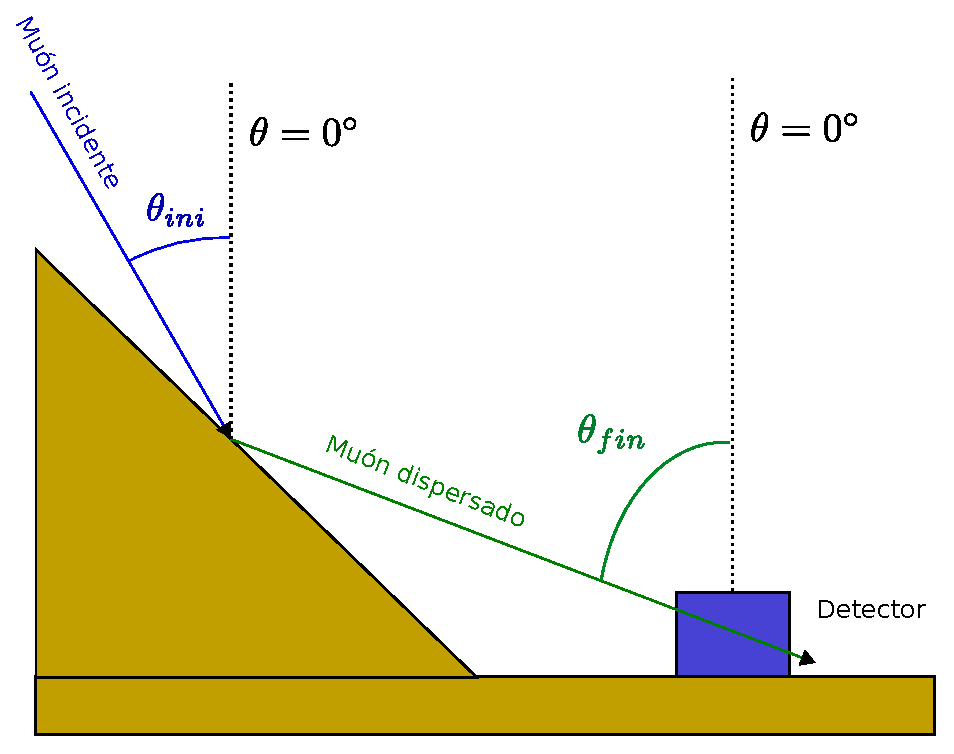
\includegraphics[width=0.6\textwidth]{Figures/imagenes/Muon_scattering.eps}
        \caption*{\textbf{Fuente.} \cite{jesusP}. }
        \label{Scattering}
    \end{center}
\end{figure}


\subsection{Partículas de trayectoria inversa}

Otra fuente de contaminación en la muografía son las partículas que impactan en el detector desde la parte posterior\footcite{Nishiyama2014}, creando trayectorias similares a los mounes provenientes desde la estructura escaneada. Ver Fig. \ref{Albedo}.

\begin{figure}[H]
    \begin{center}
        \caption[Evento falso debido a un muón que incide por la parte posterior del detector]{Evento falso debido a un muón que incide por la parte posterior del detector.}
        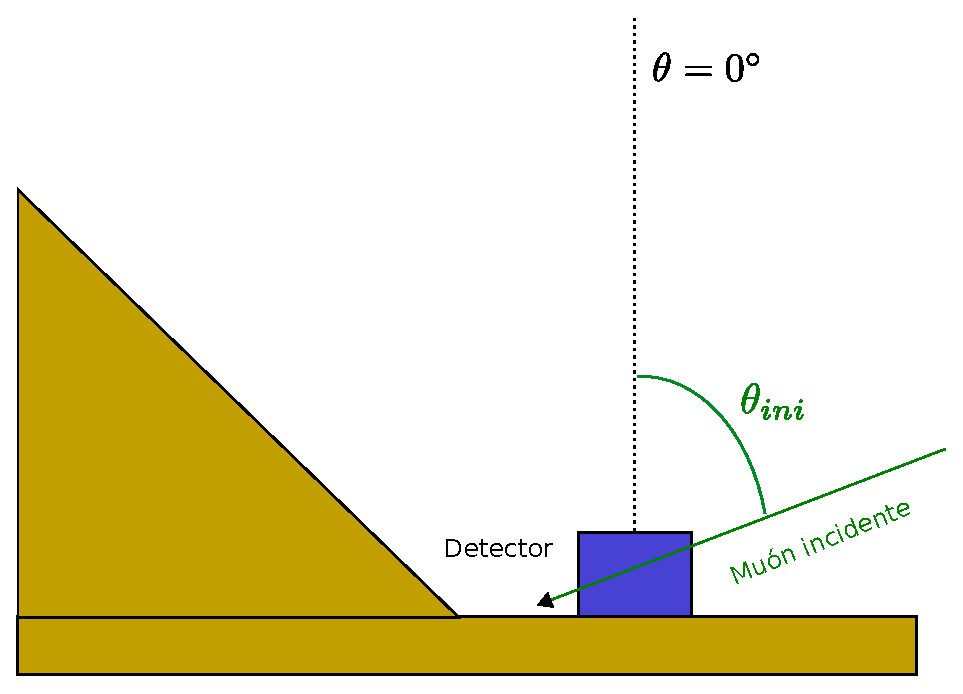
\includegraphics[width=0.6\textwidth]{Figures/imagenes/Albedo.eps}
        \caption*{\textbf{Fuente.} \cite{jesusP}. }
        \label{Albedo}
    \end{center}
\end{figure}

 
Los flujos traseros se detectan cuando la parte posterior del telescopio está expuesta a un amplio volumen de atmósfera ubicado por debajo del nivel de medición, como se observa en la Fig. \ref{topograf}. El análisis de datos discutido por Jourde et. al. \footcite{jourde2013experimental}, demuestra la existencia de un flujo de mounes traseros cuyas trayectorias podrían confundirse con la de los mounes descendentes que cruzan el volcán.


\begin{figure}[H]
    \begin{center}
        \caption{Resultado de la tomografía de alta definición en el Monte La Soufriere, sin corrección de flujo ascendente (Arriba) y con corrección de flujo ascendente (Abajo). Densidad de roca en $g.cm^{-3}$ }
        \includegraphics[width=0.65\textwidth]{Figures/imagenes/tomografia.png}
        \caption*{\textbf{Fuente.} \cite{jourde2013effects}. }
        \label{topograf}
    \end{center}
\end{figure}


Se reporta que los muones posteriores superan a los frontales dos a uno, respectivamente \footcite{jourde2013experimental}. El ruido inverso disminuye al aumentar el ángulo de elevación del telescopio. 

\subsection{Componente electromagnética}
 
Otra fuente de contaminación en la muografía ocurre a las partículas secundarias generadas por EAS entre la estructura y el detector. El flujo de PS a nivel del suelo está conformado principalmente por $\mu^{\pm}, e^{\pm}$ y $\gamma$ \ref{EAS}.

\begin{figure}[H]
    \begin{center}
        \caption[Detección de un evento falso debido a la incidencia de un $e^-$ generado en una EAS entre el objeto escaneado y el detector]{Detección de un evento falso debido a la incidencia de un $e^-$ generado en una EAS entre el objeto escaneado y el detector.}
        \includegraphics[width=0.65\textwidth]{Figures/imagenes/EAS.eps}
        \caption*{\textbf{Fuente.} \cite{jesusP}. }
        \label{EAS}
    \end{center}
\end{figure}

Las partículas secundarias generan falsa información de dos maneras:

\begin{itemize}
    \item Mediante la coincidencia accidental de dos o más partículas incidentes en el detector lo cual imita una trayectoria generada por un muón \footcite{KUSAGAYA2015}.
    
    \item Un electrón/positrón con energía suficiente para atravesar todo el detector.
\end{itemize}
    
Teniendo en cuenta que la muografía calcula la distribución densidad interna de la estructura dependiendo del flujo diferencial de los mounes que la atraviesan, un aumento en el flujo registrado debido a los eventos falsos repercute en la medición de la densidad de la estructura. \footcite{Nishiyama2014}.  

\subsection{Incidencia múltiple de partículas}
El ruido combinacional es causado por varias partículas individuales que golpean los paneles sensibles, confundiendo al detector como si fuera un evento generado por una única partícula (Ver Fig. \ref{Mult}). Estos eventos tienen la singularidad que las partículas están correlacionadas temporalmente, ya que son producidas por la misma EAS \footcite{jesusP}. 


\begin{figure}[H]
    \begin{center}
        \caption{Electrones  generados por una EAS, causando un evento de múltiple partícula que imita un evento causado por una partícula única.}
        \includegraphics[width=0.65\textwidth]{Figures/imagenes/50.png}
        \caption*{\textbf{Fuente.} \cite{jesusP}. }
        \label{Mult}
    \end{center}
\end{figure}

El retardo en promedio de los muones para una distancia al centro de la EAS menor a 1km es $<$ a 100 ns, se puede jugar con esos datos para combatir con el ruido combinacional. También se puede reducir aumentando el número de planos sensibles.

% Eliminación de ruido
\section{Eliminación de ruido en muografía}
 Debido a los altos niveles de ruido en la muografía generados por las diferentes fuentes antes mencionadas, la eliminación de ruido en muografía se convierte en un campo para indagar. Se han creado distintos métodos para la disminución del ruido en la muografía, algunos que sobresalen son la adicción de capas del material absorbente, el aumento de capas sensibles y la medición del ToF. Estos se pueden clasificar en métodos activos y pasivos.  

\begin{figure}[H]
    \begin{center}
        \caption{(Arriba a la izquierda) Muón falso. Causado por un hadrón de EAS (Arriba a la derecha) Ruido combinatorio. (Abajo a la izquierda) Muón de bajo momentum. (Abajo a la derecha) Muón de de trayectoria inversa }
        \includegraphics[width=0.86\textwidth]{Figures/imagenes/noise.jpg}
        \caption*{\textbf{Fuente.} \cite{bonechi2020atmospheric}. }
        \label{ruido}
    \end{center}
\end{figure}


\subsection{Métodos activos}

Estos métodos buscan la eliminación de fuentes de ruido mediante el análisis de los datos entregados, para encontrar un patrón que muestre el comportamiento del los eventos falsos.

L. Oláh et. al. \footcite{olah2018high} implementaron siete detectores tipo cámara proporcional de múlti-hilo (MWPC), con un tamaño de ($ 80 \times 80$ cm$^{2}$), con cinco láminas de protección contra la radiación construidas de plomo, cada placa está oculta dentro de otra caja de acero inoxidable para protegerla mecánicamente y evitar la exposición a la toxicidad del plomo. La Fig. \ref{multi} muestra el detector desde una vista lateral.

 Debido a la buena resolución espacial, la dispersión de partículas de baja energía en las placas de plomo se puede medir a lo largo de la trayectoria y, por lo tanto, estas partículas de fondo $< 2$ GeVc$^{-1}$ se pueden eliminar de los datos registrados. 
 
  
  \begin{figure}[H]
    \begin{center}
        \caption{El sistema de observación muográfica basado en MWPC (mMOS). La vista esquemática de mMOS que consta de siete cámaras proporcionales multi-hilo y cinco placas de blindaje de plomo con un grosor de 2 cm cada una }
        \includegraphics[width=0.6\textwidth]{Figures/imagenes/multi.png}
        \caption*{\textbf{Fuente.} \cite{Olh2018}. }
        \label{multi}
    \end{center}
\end{figure}
Dentro de los métodos activos se encuentra la medición del tiempo de vuelo (ToF). EL ToF es el tiempo que tarda una partícula en recorrer una distancia determinada. Con esta  estimación se pueden calcular otras variables como velocidad, momento, dirección e identidad. 
El momento \textit{p} se relaciona con el ToF mediante:

\begin{equation}
    p= \frac{m_ocd}{\sqrt{c^2t^2-d^2}}
\label{MOM}
\end{equation}

Donde $m_o$ es la masa de la partícula cargada en reposo, c es la velocidad de la luz, d es la distancia recorrida y t es el tiempo de vuelo. 

% Parte del párrafo que cita la imagen.

La Fig. \ref{tof} muestra el ToF en función del ángulo cenital, las elipses sólidas identifican a los muones que se propagan hacia abajo (componente principal del flujo), las elipses discontinuas muestran la existencia de muones con propagación hacia arriba identificadas por el detector. Los resultados para la medición presentada en la figura muestran que la contaminación asciende al 70$\%$ del flujo total, y disminuye al 30$\%$ en ángulos de -10° y en cero por encima de -20°. Estos resultado permiten corregir las imágenes obtenidas por el detector \footcite{Marteau2014}.


 \begin{figure}[h]
    \begin{center}
        \caption{Distribución del ToF en función del ángulo cenital para los datos registrados en el volcán La Soufriere. El horizonte está representado por la línea discontinua. Las elipses sólidas azul y roja muestran respectivamente los eventos hacia atrás ($\alpha_{B}  < 0 $  y $\bigtriangleup t < 0$ ) y hacia adelante ($\alpha_{F} < 0$ y $\bigtriangleup t > 0$) correspondientes a los flujos descendentes. Las elipses discontinuas muestran eventos correspondientes a muones ascendentes desde adelante (elipse roja, $\alpha_{B} < 0$ y $\bigtriangleup t > 0$) y hacia atrás (elipse azul, $\alpha_{F} < 0$ y $\bigtriangleup t <0$) }
        \includegraphics[width=0.57\textwidth]{Figures/imagenes/ToF.png}
        \caption*{\textbf{Fuente.} \cite{jourde2013effects}. }
        \label{tof}
    \end{center}
\end{figure} 
 
\subsection{Métodos pasivos}
Este método consiste en adicionar capas de material absorbente entre los paneles del hodoscopio. Lo que se busca es que la partícula que atraviesa el detector pierda toda su energía en el material absorbente.
La primera implementación de esta técnica fue hecha por Nagamine et. al. \footcite{Nishiyama2014}, donde introducen dos placas absorbentes de hierro (40 g/cm$^{2}$) dentro del sistema de detección para filtra los muones de baja energía ($< 1 GeVc^{-1}$).

 

 % Estado del arte.
\chapter{ \MakeUppercase{El Detector MuTe}}
El telescopio de muones (MuTe) es un detector creado para realizar muografía de volcanes en Colombia. Tiene como característica principal separar los mounes que ingresan al detector de las fuentes de ruido que afectan la muografía. Aplica dos técnicas para el reconocimiento de partículas: la medición del ToF de partículas incidentes y la pérdida de energía.
MuTe esta compuesto por dos detectores: un hodoscopio y un detector Cherenkov de agua (WCD).\\

\begin{figure}[h!]
\begin{center}
\caption{Vista lateral del detector. El WCD contiene 1.7$m^3$ de agua y se ubica sobre el soporte de elevación. El hodoscopio compuesto por dos paneles centelladores de
120 cm × 120 cm ubicados dentro de cajas metálicas que los protegen de la contaminación lumínica y de la humedad.}
\includegraphics[width=1 \textwidth]{Figures/imagenes/26.png}
\caption*{\textbf{Fuente.} \cite{jesusP}. }
\label{detectores}
\end{center}
\end{figure}


El hodoscopio está conformado por dos paneles sensibles, cada panel contiene 30 barras centelladoras verticales y 30 horizontales, creando una matriz de 900 píxeles. El hodoscopio de MuTe es un dispositivo de conteo de sucesos y su principal función es la estimación del flujo de muones.\\

El WCD es un tanque de acero que contiene 1,7 $m^3$ agua y un tubo fotomultiplicador como elemento sensible. Este detector mide la energía recibida por las partículas cargadas y permite diferenciar los eventos registrados en: muones, electrones/positrones y múltiple partícula.\\

El Sistema ToF de MuTe permite estimar el tiempo que tardan las partículas en atravesar el hodoscopio en una distancia dada y la dirección de estas. Este permite filtrar las partículas que ingresan por la parte posterior. Con el ToF y la energía depositada en el WCD MuTe estima el momentum de las partículas incidentes.

\section{Flujo de datos}

Los datos adquiridos por MuTe son sincronizados temporalmente por un GPS y guardados en dos discos duros, uno para los datos del hodoscopio y otro para los datos del WCD. Cada hora se crean nuevos archivos que almacenan 1 hora de datos. Los datos almacenados tiene meta-datos de presión atmosférica, temperatura y el consumo energético para hacer correcciones de flujo y evaluar la autonomía del detector. Cabe resaltar que estimación del momentum se hace offline.\footcite{jesusP}.
 % Mute
%\chapter{\MakeUppercase{Metodología}}
\label{ch:e_lento}


\subsection{Extracción de características. \\ \\}

Se busca realizar una parametrización y análisis de los datos suministrados por el WCD por medio de un histograma de carga. A continuación se presentan los pasos empleados:

\begin{itemize}
    \item Extraer los datos crudos del detector y posteriormente ordenarlos.
     \item Parametrizar los datos para ajustarlo a una distribución probabilística.
     \item Implementar un histograma de carga, para identificar y separar la componente muónica de la electromagnética y multipartícula.
     \item Encontrar características según los resultados de las variables de entrada de cada componente.
 \end{itemize}
 

\subsection{Ajuste de características para desarrollar clasificadores supervisados que discriminan entre mounes, EM y multipartícula. \\ \\}

Se va a identificar las características para ajustarlas a diferentes modelos de clasificación y etiquetarlas entre las componentes estudiadas en el proyecto. A continuación se presentan las actividades correspondientes:
\begin{itemize}
    \item Definir una función de probabilidad optimizando los valores que ajusten a la curva de la distribución seleccionada.
    \item A partir de los valores ajustados con la función de densidad de probabilidad (PDF), analizar independientemente cada componente por medio de la distribución extraída del histograma de carga.
    \item Evaluando las componentes independientes, se etiqueta cada tupla de datos con unos y ceros, mounes y EP respectivamente.
    \item Para el entrenamiento de los datos con el modelo a emplear, se usan características y etiquetas, de tal manera que se pueda evaluar el comportamiento del clasificador a usar\footcite{perez2005modelos}.
\end{itemize}

\subsection{Implementación del clasificador no supervisado para discriminar los mounes de bajo momentum.\\ \\}

Se comprueban algoritmos no supervisados de clasificación usando previamente la discriminación de la componente electromagnética de la muónica, para separar ahora entre muón de alto y de bajo momentum ($<$ 1 GeV/c). Este proceso se llevará a cabo después de comparar sus tiempos de vuelo como característica.  \\



\subsection{Comparación y validación de todos los datos obtenidos a lo largo del proyecto de investigación.\\ \\ }

Esta fase final divide en:

\begin{itemize}
    \item Comparación de los clasificadores supervisados por métricas de precisión.
    \item Analizar los datos obtenidos por los clasificadores no-supervisados con métricas de precisión.
    \item Encontrar y diferenciar el mejor resultado de cada clasificador, optimizando el resultado.
\end{itemize}

 % Metodologia
\chapter{ \MakeUppercase{Clasificación supervisada de ruido en muografía por pérdida de energía.}}
\label{ch:e_rapido}

En esta sección se muestra la clasificación de los eventos detectados por MuTe mediante algoritmos de aprendizaje supervisado. En este apartado se hace un recuento de los métodos y propuestas que se emplearon para concluir la primera etapa, con los resultados y los problemas que surgieron durante su desarrollo.

\section{Extracción de características.}

La extracción de características se basa en la parametrización y análisis de los datos suministrados por el WCD por medio de un histograma de carga. A continuación se presentan los pasos empleados:

\alglanguage{pseudocode}
\begin{algorithm}[h]
\small
\caption{Extracción de características}
\label{Begin_Read}
\begin{algorithmic}[1]
\State Extraer los datos crudos del detector y posteriormente ordenarlos.
\State Parametrizar los datos para ajustarlo a una distribución probabilística.
\State Implementar un histograma de carga, para identificar y separar la componente muónica de la electromagnética y multipartícula.
\State Encontrar características según los resultados de las variables de entrada de cada componente.
\Statex
\end{algorithmic}
  \vspace{-0.1cm}
\end{algorithm}

 
\section{Discriminación entre muones, componente electromagnética\\ y multi-partícula.}

Las características (la carga de las componentes, la variaza y la media) se ajustan a diferentes modelos de clasificación como: \textit{naive gaussian}, \textit{suport vector machine}, \textit{random forest} y \textit{gaussian mixture model}. Se etiquetan como componente: muónica, electromagnética y multi-partícula. Para ello se emplearon los siguientes pasos:

\alglanguage{pseudocode}
\begin{algorithm}[h]
\small
\caption{Discriminación entre muones, electromagnética y multi-partícula.}
\label{Begin_Read}
\begin{algorithmic}[1]
\State Definir una función de probabilidad optimizando los valores que ajusten a la curva de la distribución seleccionada.
\State A partir de los valores ajustados con la función de densidad de probabilidad (PDF), analizar independientemente cada componente por medio de la distribución extraída del histograma de carga.
\State Se etiqueta cada tupla de datos que se  representan como: 1 para mounes, 0 para electromagnético y 2 para multi-partícula.
\State Para el entrenamiento de los datos se emplean los siguientes modelos de clasificación: \textit{naive gaussian}, \textit{suport vector machine}, \textit{random forest} y \textit{gaussian mixture model}. Donde se utilizan las características (la carga de las componentes, la variaza y la media) y etiquetas, de tal manera que se pueda evaluar el comportamiento del clasificador a usar\footcite{perez2005modelos}.
\Statex
\end{algorithmic}
  \vspace{-0.1cm}%
\end{algorithm}


\section{Minería de datos}
Inicialmente la base del problema se encuentra en el reconocimiento de los datos entregados por el WCD. Los datos están dados por los valores de carga (energía depositada). Los datos se modelaron con histogramas de frecuencia de carga, de dos dimensiones (Carga vs Frecuencia), como se muestra en la Fig. \ref{uno}. El histograma evidencia tres componentes, que guiados por un conocimiento a priori, se clasifican como (muónica, electromagnética y multi-partícula).\\

%Se cargan los datos crudos implementando histogramas donde se proyecta la cantidad de datos.
%-El modelo fue creado a partir de los datos de carga con el histograma de Frecuencia de la Carga (eje X), simulando los datos crudos (llamados \textit{Carga1}), ya que, al inicio del proyecto no se contaba estos. Cabe resaltar que se hizo la prueba del modelo, se obtuvieron resultados y de estos resultados, conclusiones. Todo esto a partir de los datos crudos de Carga.-\\ 

\begin{figure}[h!]
\begin{center}
\caption {Histograma de carga para un registro de datos de una hora del WCD de MuTe. (arriba).  Datos del WCD de eventos que han atravesado el hodoscopio (abajo).}
\includegraphics[width=0.7
\textwidth]{Figures/imagenes/1.png}
\label{uno}
\end{center}
\end{figure}

Al recibir los datos crudos totales, se hizo el procesamiento y modelamiento de los datos para implementarlos en el modelo GMM ya ajustado con los datos de carga del histograma. El modelo presentó complicaciones para evidenciar las componentes, esto se presentó debido a un grupo de datos innecesarios (outliers). Separando y visualizando los datos crudos, se estableció un límite donde sólo se tuvo en cuenta valores de carga $<$ 800 ADC.bin, ya que por encima de esto los datos no aportaban información relevante (ver Fig. \ref{dos}).

\begin{figure}[h]
\begin{center}
\caption{Datos de Carga crudos. ARRIBA: Datos completos de carga.  ABAJO:.Datos acotados por el umbral (Carga $<$ 800)}
\includegraphics[width=0.6\textwidth]{Figures/imagenes/2.png}
\label{dos}
\end{center}
\end{figure}


\section{Modelo de mezcla de gaussianas y parametrización}

Los modelos de mezcla gaussiana (GMM), representan subpoblaciones normalmente distribuidas dentro de una población general. Este modelo parametriza un subconjunto que pertenece a un grupo de datos. GMM puede tener más de 2 componentes y estima los parámetros individuales para modelar por medio de distribuciones normales.

GMM necesita parámetros iniciales para obtener un mejor ajuste. Los parámetros más usados en este caso fueron: el número de componentes, el peso de cada una de las componentes, el número de inicializaciones que debe hacer y el número de iteraciones. Cuando el GMM converge retorna valores como las medias, varianzas y el peso de cada una de las componentes. Adicionalmente, se ajustó una PDF a cada componente, (muónica, electromagnética y multi-partícula) permitiendo comparar los resultados con los datos. 

En la primera separación de las componentes se evidenció que el modelo con pocos datos (1.323) no responde acertadamente. Pero al contar con la cantidad total de los datos (1'273.125), el modelo mostró un mejor ajuste. 

\begin{figure}[h!]
\begin{center}
\caption{Histograma de frecuencia con los datos y la función de densidad de probabilidad ajustada por GMM. Con las medias calculadas, para apreciar el ajuste a los datos.}
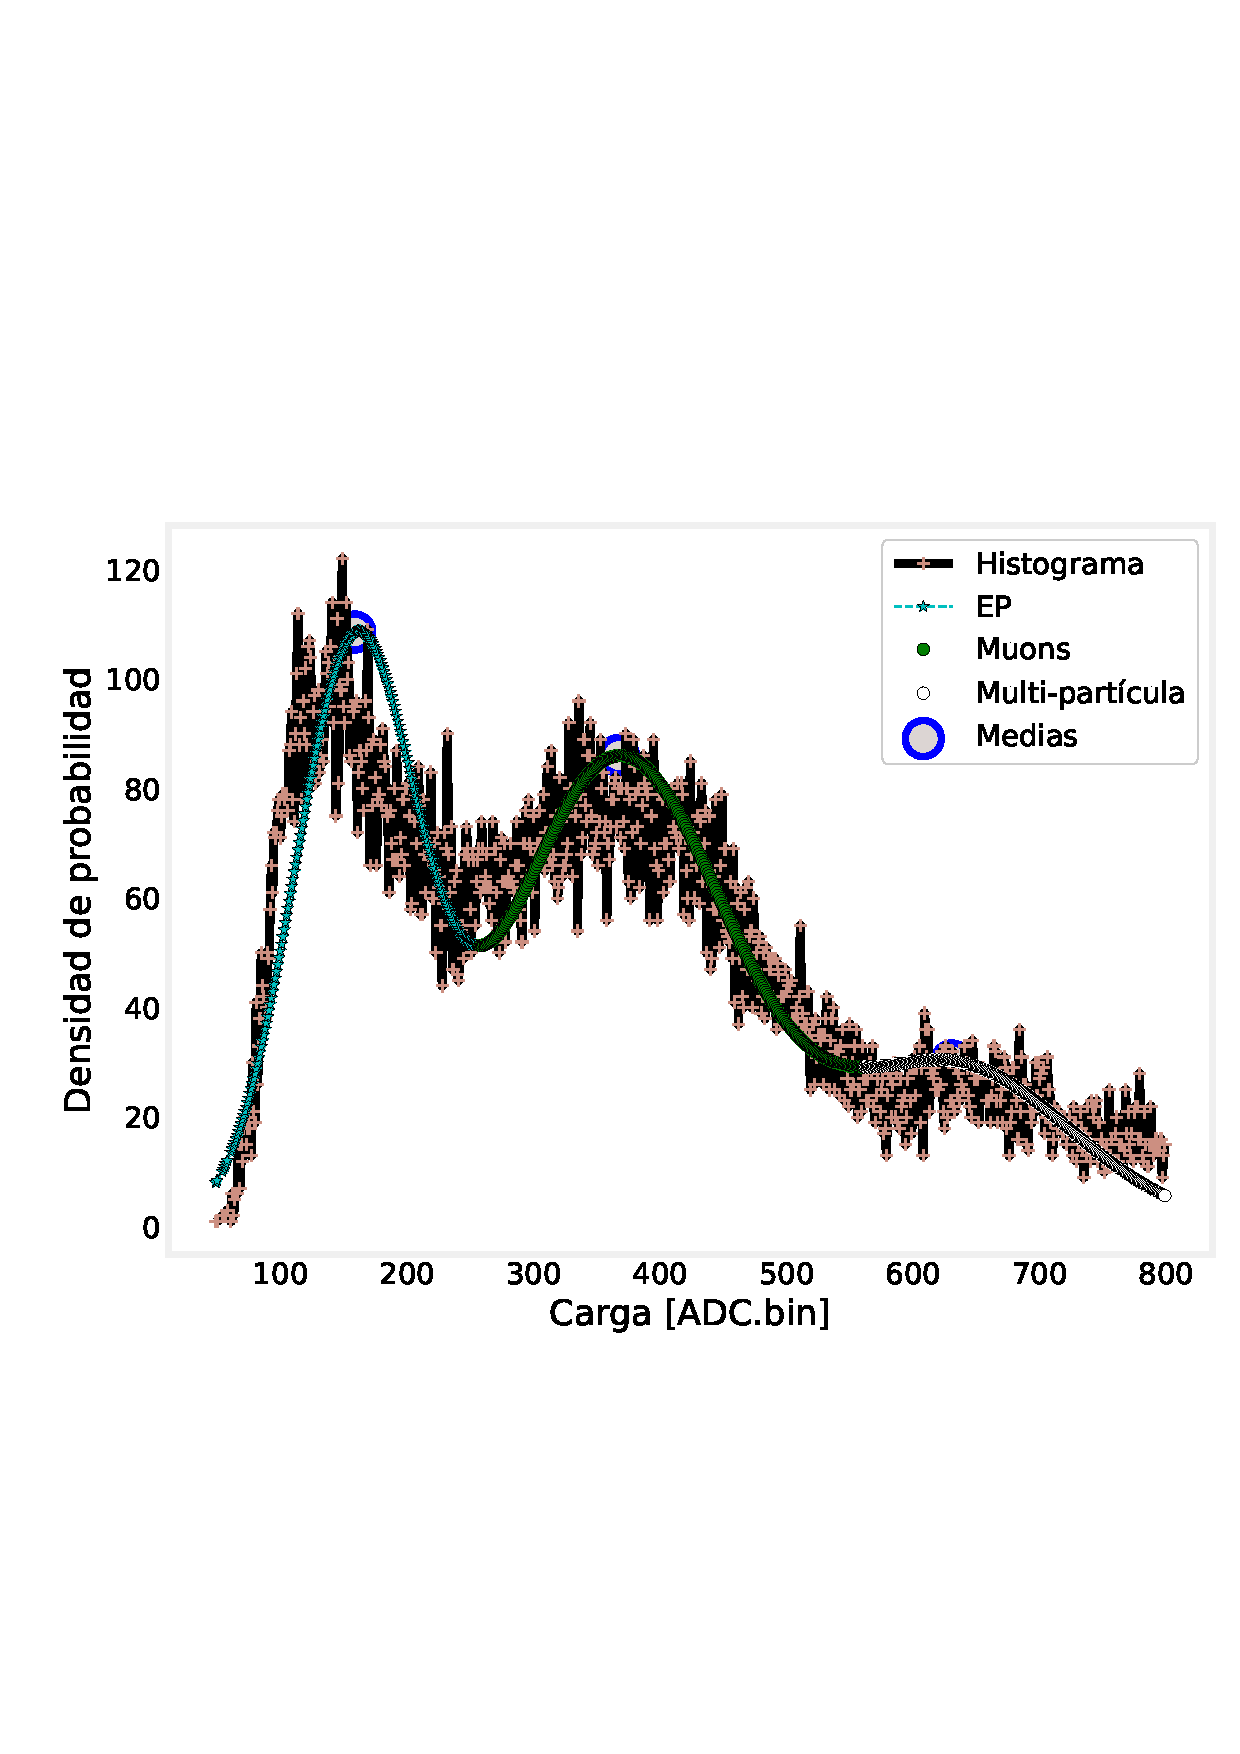
\includegraphics[width=0.7\textwidth]{Figures/imagenes/4.png}
\label{cuatro}
\end{center}
\end{figure}

%Los primeros datos procesados fueron \textit{Carga1}, que cumplían la función de entregar valores de carga, pero no había valores repetidos, puesto que se extraían del histograma de frecuencia limitando y confundiendo a GMM. Todo el modelo se construyó con los datos de \textit{Carga1} (al principio del proyecto)ver Fig.\ref{tres}, se hizo para tener una base al momento de agrupar todos los datos reales, para ajustar el modelo al ingresar los datos de \textit{Carga2}. ver Fig. \ref{cuatro}.%

%Con los resultados obtenidos de GMM se pudo avanzar de una formas más fácil y precisa, ya que se parametrizaron cada una de las gaussianas para un manejo independiente mejorando el análisis a lo largo del proyecto. %


\section{Construcción de gaussianas y etiquetado}

Con los parámetros de cada una de las gaussianas obtenidos previamente, se creó una función gaussiana definida por la Ecuación (\ref{P.D.F}) de densidad de probabilidad.
\begin{equation}
f(x)=A*e^{-\frac{1}{2}(\frac{x-\mu}{\sigma})^2}
\label{P.D.F}
\end{equation}
donde A es la escala, $\mu$ la media, $\sigma$ la varianza y x los datos. Se definieron tres funciones para las tres componentes (EP, muón y multi-partícula) como se muestra en la Fig. \ref{cinco}


Definidas las tres funciones se analizan independientemente etiquetando: 0 para muon, 1 para electromagnético y 2 para multi-partícula. Se crea un vector con las etiquetas de la misma longitud del vector carga.

\begin{figure}[h!]
\centering
\begin{center}
\caption{ Las tres componentes: la muónica (verde),  la electromagnética (azul) y multi-partícula (roja), representadas por su respectiva función de densidad de probabilidad.}
\includegraphics[width=0.7\textwidth]{Figures/imagenes/5.png}
\label{cinco}
\end{center}
\end{figure}
\section{Clasificación supervisada, división y entrenamiento}\\

Con los datos etiquetados se debe hacer un \textit{Split} para entrenar el clasificador. En este proyecto se usó \textit{Train Test Split} implementado en la librería de \textit{SKlearn}, ya que además de cumplir con el objetivo principal es una herramienta fácil y rápida de usar. Los datos fueron separados en dos conjuntos, Test (70\% de datos) y train (30\% de datos) para evaluar los modelos de clasificación. \\

En este caso se usaron tres modelos de clasificación supervisada: \textit{Naive Gaussian, RandomForest y Support Vector Machines} implementados en la librería \textit{SKlearn}. Los clasificadores se evaluaron mediante métricas de la matriz de confusión y eficiencia. Se generaron visualizaciones gráficas. (ver Fig. \ref{seis}).\\
\\

\begin{figure}[h]
\begin{center}
\caption{Resultados del etiquetado de los datos por el clasificados y ajuste de las distribuciones.}
\includegraphics[width=0.8\textwidth]{Figures/imagenes/6ta.png}

\label{seis}
\end{center}
\end{figure}\\


En la matriz de confusión de la Tabla (\ref{mat}) se muestra el resultado obtenido por el clasificador. Los valores erróneos se dan entre las componentes estrictamente contiguas, como lo es la electromagnético con muónica y la muónica con la multi-partícula. No hubo fallos en la predicción entre muón y multi-partícula. \\

\begin{table}[t]
\begin{center}
\caption{Matriz de confusión del \textit{naive gaussian}. Donde las columnas 1, 2 y 3 son valores reales que representan las componentes: electromagnética, muónica y multi-partícula. Las filas 1, 2 y 3 son los valores predichos que definen las componentes electromagnética, muónica y multi-partícula.}
\begin{tabular}{| c | c | c | c | }
\hline
 & Electromagnética & Muón & Multi-partícula\\
 \hline
 Electromagnética & 4026 & 49 & 0\\
\hline
 Muón & 0 & 5297 & 0\\
\hline
Multi-partícula & 0 & 51 & 1702 \\
\hline

\end{tabular}
\label{mat}
\end{center}
\end{table}


El valor de precisión en la Tabla (\ref{pres}) se refiere a cuán cerca del valor real se encuentra el valor medido. En la componente electromagnética y multi-partícula se obtuvo una precisión de 100\%. La muónica se redujo a 98\%: predijo que 49 datos de carga pertenecían a la componente muónica, cuando realmente pertenecían a la componente electromagnética y en 51 casos el clasificador los etiquetó como muónica cuando pertenecía verdaderamente a la componente multi-partícula.

La veracidad o sensibilidad del modelo determina la proporción de los casos positivos clasificados por el modelo con respecto al total de los datos positivos. En esta métrica el clasificador asignó correctamente el 100\% de los datos pertenecientes a la componente muónica. En la componente electromagnética (99\%) obtuvo 4026 verdaderos positivos y 49 falsos positivos (muónica). En la multi-partícula (97\%) se obtuvieron 1702 verdaderos positivos y 51 falsos positivos (muónica).  


\begin{table}[t]
\begin{center}
\caption{Precisión extraídas de la matriz de confusión}
\begin{tabular}{| c | c | c | c | c |}
\hline
 & Precisión & Veracidad & score & Datos \\ \hline
Electromagnético & 1.00 & 0.99 & 0.99 & 4075 \\ \hline
Muón & 0.98 & 1.00 & 0.99 & 5297 \\  \hline
Multi-partícula & 1.00 & 0.97 & 0.99 & 1753 \\\hline

\end{tabular}
\label{pres}
\end{center}
\end{table}





 % Clasificación supervisada
\chapter{\MakeUppercase{Clasificación no supervisada de ruido combinacional por medio del tiempo de vuelo}}

En este apartado se analizaron los eventos detectados por MuTe mediante las mediciones del ToF y GMM. Los eventos se clasifican como correlacionados y no correlacionados por medio del tiempo de vuelo (ToF).  Las partícula correlacionadas e individuales su tiempo de vuelo oscila entre 2 a 30$ ns$, mientras que las partículas no correlacionadas, la diferencia temporal entre las 2 partículas es $> 300 ns$, revisar Fig. \ref{placas}. La probabilidad de que ocurra un evento por partículas no correlacionadas con un diferencia temporal $<  200ns$ es de $\med 0,05\%$ \footcite{jesusP}.

\begin{figure}[h!]
\begin{center}
\caption{Partículas incidentes que cruzan los paneles. Estos se clasifican en correlacionados (verde oscuro), no correlacionados (verde claro), y eventos simples (rojo).}
\includegraphics[width=0.71\textwidth]{Figures/imagenes/panel.png}
\label{placas}
\end{center}
\end{figure}

\section{Eventos de partícula simple, correlacionados y no-correlacionados teniendo en cuenta el ToF }


\subsection{Tratamiento y análisis de datos.\\}

Inicialmente, se hizo una visualización de los datos para analizar la relación que tienen los eventos con las etiquetas teniendo en cuenta la información a-priori. La primera gráfica muestra el tiempo de vuelo de cada uno de los eventos. En la Fig. \ref{300} se observa una aglomeración de datos correspondientes a los eventos correlacionados (ToF < 300ns). Los no correlacionados se dispersan uniformemente sobre los valores > 300ns.

El histograma de frecuencia, evidencia la distribución de los eventos con ToF $< 300 ns$, como se muestra en la Fig. \ref{ocho}.\\

\begin{figure}[h!]
\begin{center}
\caption{ Tiempo de vuelo de cada evento. Un umbral en 300ns (linea negra) permite dividir los eventos correlacionados (< 300ns) de los no-correlacionados (> 300ns).}
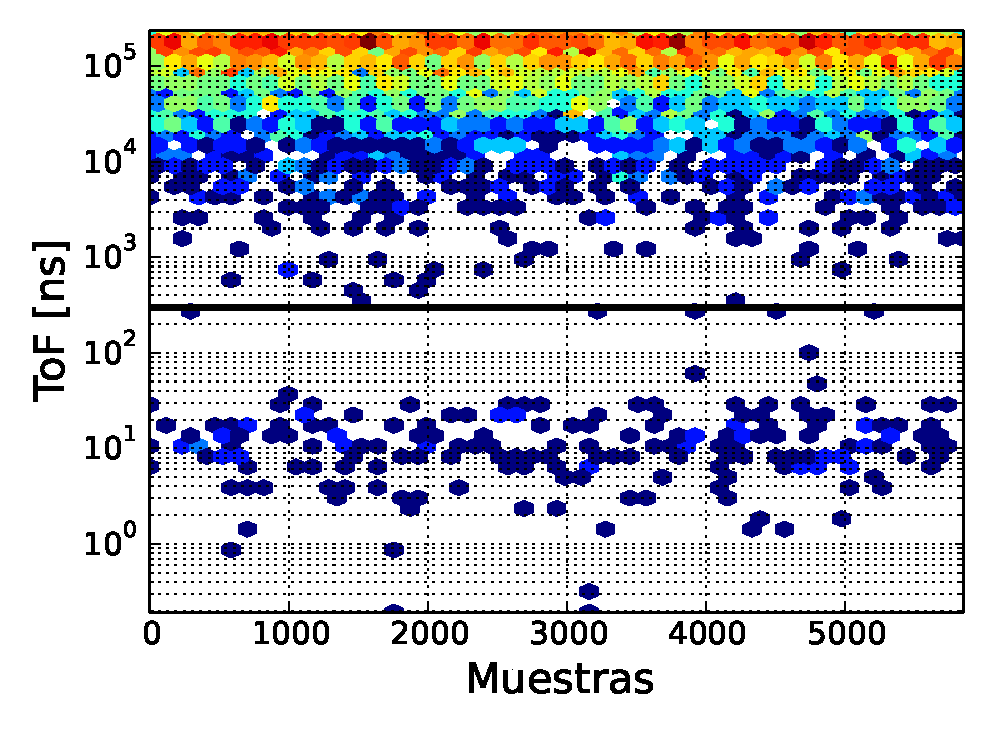
\includegraphics[width=0.7\textwidth]{Figures/imagenes/ag.eps}
\label{300}
\end{center}
\end{figure}


También se visualizaron los datos en orden logarítmico para corroborar la conclusión obtenida de las dos gráficas anteriores. En la Fig. \ref{nueve}, se evidencia una concentración de muestras alrededor de 10 ns corroborando un mayor número de eventos correlacionados. Ubicadas estas zonas de interés, se parametrizan los datos por medio de distribuciones.\\



\begin{figure}[h!]
\begin{center}
\caption{ Histograma de frecuencia de los datos del tiempo de vuelo.}
\includegraphics[width=0.7\textwidth]{Figures/imagenes/7.png}

\label{ocho}
\end{center}
\end{figure}

\begin{figure}[h!]
\begin{center}
\caption{Tiempo de vuelo en orden logarítmico. Se distinguen los eventos de partícula simple y correlacionadas con un ToF menor a 300ns, mientras que los eventos no correlacionados tienen ToF mayores a 300 ns  }
\includegraphics[width=0.6\textwidth]{Figures/imagenes/8.png}

\label{nueve}
\end{center}
\end{figure}


\section{Clasificación y segmentación.}
 Bajo las métricas del ToF se ingresaron los datos a GMM para parametrizar cada componente. Se trabajó con 5883 datos definiendo parámetros iniciales como: el número de componentes (2), el número de iteraciones (1000), los pesos de cada componente (0.9 para correlacionados y 0.1 para no-correlacionados) y el número de iniciaciones que tuvo el modelo (5). Todo escogido para que se ajustara mejor a los eventos de partícula simple y correlacionada.
 
 Al parametrizar las componentes, se validó el modelo con los datos reales. De los parámetros de salida se tomó la varianza (76.80), la media (10.22) y los pesos de las componentes (0.96 y 0.037) para empezar con la separación de los eventos correlacionados y la eliminación de los no-correlacionados. Como se ve en la Fig. \ref{diez}).\\
 \\
 \\


\begin{figure}[h!]
\begin{center}
\caption{ToF $< 300  ns$. Eventos correlacionados. Los datos entregados por el detector y el modelo ajustado, muestran que los eventos se concentran en un ToF menor a 40ns.}
\includegraphics[width=0.75\textwidth]{Figures/imagenes/9.png}

\label{diez}
\end{center}
\end{figure}

\chapter{CLASIFICACIÓN NO SUPERVISADA DE LOS MUONES DE BAJO MOMENTUM.}
Para la discriminación de los muones de bajo momentum (<1 GeV/c), se trabajó con la relación de dos variables: el momento y el ToF. Se graficó en escala logarítmica para ver la relación entre las 2 variables e identificar su umbral.  Los muones con momento menor a $1 GeV/c$ son filtrados ya que sufren una dispersión angular que afecta la resolución espacial del MuTe. El proceso de clasificación se llevó a cabo gracias a algoritmos de clasificación no supervisada.


\section{Manejo de variables}

Inicialmente se eliminaron datos NaN de los datos crudos que dificultaban el procesamiento. Los datos resultantes se redujeron $\sim$ en un 40$\%$. En esta parte del proyecto ya se filtró la mayoría de las fuentes de ruido. 
Tras relacionar el ToF y el momentum, ver Fig.(\ref{doce}), se clasificó los muones de interés que presentan un momentum mayor a 1GeV/c. A continuación se explica la relación entre el ToF y el momento.\\ 

\begin{figure}[h!]
\begin{center}
\caption{ToF vs momentum. El 54$ \%$ de las partículas tiene momentum mayor a 1GeV/c (linea púrpura).}
\includegraphics[width=0.75\textwidth]{Figures/imagenes/11.png}

\label{doce}
\end{center}
\end{figure}

\section{Estimación de momentum}
El sistema de ToF de MuTe mide el tiempo de vuelo que tardan las partículas cargadas de energía en atravesar un determinada trayectoria en el hodoscopio. Utilizando el ToF y la energía depositada en el WCD, MuTe estima el momentum de todas las partículas que ingresan al detector, estableciendo umbral para discriminar las partículas de baja energía (< 1Gev/c) \footcite{jesusP}.

La estimación del momentum se lleva a cabo con el fin de encontrar los eventos que sufren de dispersión múltiple. El cálculo del momentum depende de 2 variables, el ToF y la distancia recorrida entre las placas, que se define en la Ecuación ( \ref{MOM}).

\section{Clasificación}

En el proceso de clasificación se probaron varios métodos: \textit{Aglomerative Clustering}  \textit{Kmeans}, \textit{PCA} y \textit{ Spectral Clustering} . Con \textit{Aglomerative Clustering} y \textit{Kmeans} hubo un mejor ajuste de los datos, como se ve en la Fig. (\ref{ACvskM}). 
Luego estos clasificadores se probaron con diferente número de clúster, para compararlos minuciosamente mediante la medición de la precisión. \\




\section{\textbf{Análisis de Resultados.}}

\begin{figure}[h!]
\begin{center}
\caption{ToF vs momento entregados por los clasificadores \textit{AgglomerativeClustering} y \textit{Kmeans}, se muestra la comparativa de 2 a 4 clusters, con el umblar en 1GeV/c. (linea roja)}
\includegraphics[width=0.9\textwidth]{Figures/imagenes/AK.png}
\label{ACvskM}
\end{center}
\end{figure}

Para la decisión final se tuvo en cuenta 2 factores: la precisión de la clasificación y la complejidad computacional.  En este orden de ideas, según los resultados obtenidos se escogieron tres clústeres con el algoritmo de \textit{Aglomerative Clustering}. Al aumentar el volumen de datos y el número de clústeres, se afecta el funcionamiento fluido del algoritmo, así que se validó con el resultado más óptimo.\\


\begin{figure}[h!]
\begin{center}
\caption{ToF vs momento entregados por los clasificadores \textit{Aglomerative Clustering} y \textit{Kmeans}, se muestra la comparativa de 2 a 4 clusters. Muestra el porcentaje de cada grupo en cada cluster.}
\includegraphics[width=0.9\textwidth]{Figures/imagenes/tor.png}
\label{ACvskM1}
\end{center}
\end{figure}

En términos generales $\sim$ el 90 $\%$ de los eventos estaban en la zona de aceptación (>1 GeV/c), esta condición se presento en todos los clusteres. Otra cosa que cabe mencionar, es que en todos los clusters el grupo de mayor cantidad de eventos estuvo estrictamente después del umbral de 1GeV/c como se muestra en la Fig. \ref{ACvskM}. 


% \begin{figure}[h!]
% \begin{center}
% \caption{\textit{Aglomerative Clustering} y \textit{Kmeans}, se muestra la comparativa de 2 a 4 clusters. Relaciona cada grupo con su respectivo número de muestras.}
% \includegraphics[width=0.65\textwidth]{Figures/imagenes/coin.png}
% \label{ACvskM2}
% \end{center}
% \end{figure}

No hubo diferencias significativas en los resultados entre los 2 algoritmos al evaluarse con el mismo número de clusters, diferían por  $\sim$3\% (200 datos). La diferencia a validar fue la posición del grupo en la muestra de datos. Por ejemplo en 2 clusters con \textit{Kmeans}, el grupo \textit{rojo} con 5817 datos, fue el menos preciso con respecto al umbral de 1GeV/c. Para 3 clusters se tuvo una mejor precisión, con un 94.6\% para \textit{AgglomerativeClustering} y 93.4\% para \textit{Kmeans} como se puede ver en la Fig. \ref{ACvskM1}.

 %  Clasificación no supervisada.
% ------------------------------------------------------------------------
% ------------------------------------------------------------------------
% ------------------------------------------------------------------------
%                             Conclusiones
% ------------------------------------------------------------------------
% ------------------------------------------------------------------------
% ------------------------------------------------------------------------

\chapter{CONCLUSIONES}

%EL desarrollo de esta trabajo costa de la una construcción de un conjunto de modelos de clasificación de aprendizaje automatizado que proporcionan técnicas para la discriminación de las principales fuentes de ruido de la muografía. 

Los resultados obtenidos con los modelos de mezcla gaussiana (GMM) permitieron parametrizar las componentes que conforman los eventos registrados por el detector de MuTe. El clasificador tuvo una precisión de 100 \% etiquetando los eventos pertenecientes a la componente electromagnética y multi-partícula; en la muónica fue del 98\%.\\

Con los datos del ToF se filtraron las partículas correlacionadas con un ToF < 300ns. El modelo ajustó bien a los datos ya que se presentaba una aglomeración marcada entre 0 y 50 ns. Los eventos multi-partícula no correlacionados presentaron un ToF por encima de 300\,ns.\\

%De 0 a 350 ns con un total de 256 datos, fueron 223 eventos los que se alojaron en el rango de 0 a 76 ns, los demás datos están esparcidos al lo largo de la gráfica, como se ve en la Fig. \ref{diez}. Son estos los eventos los que el modelo entiende del comportamiento de los datos y es gracias a esas características el ajuste de los datos.\\
    
%Con las mediciones del ToF, se visualizaron los datos para analizar algún patrón en los eventos.%
%Los resultados de las mediciones del ToF visualizaron una concentración de muestras alrededor de los 10 ns, donde se pudo inferir algún comportamiento. Bajo las métricos del ToF se ingresan 5883 datos definidos con parámetros iniciales como: el numero de componentes, número de iteraciones, pesos para las componentes y número de iniciaciones. Al parametrizar se ajusta un modelo con datos de salida: varianza, media y pesos de las componentes, el cual permite la segmentación de los eventos correlaciones y no correlacionados.


De las mediciones de momentum se buscó encontrar y separar los eventos que son afectados por dispersión múltiple. Se estableció un umbral para discriminar las partículas de baja energía con un momentum menor a 1\,Gev/c. En el proceso de clasificación se indagaron métodos como: \textit{Aglomerative Clustering} \textit{Kmeans}, \textit{PCA} y \textit{ Spectral Clustering}, variando el número de clusters. Encontramos que los mejores resultados están entre 2 y 4 clusters.\\

La aglomeración parcial de los datos en zonas específicas fue clave para que los algoritmos identificaran de acuerdo al número de clusters las clases. Con 3 clusters para \textit{Aglomerative Clustering} se tuvo 5511 (rojo), 8 (azul) y 304 (verde), y con \textit{Kmeans} 5441 (rojo), 6 (azul),  376 (verde). Dejando en ambos casos el grupo de mayor número de datos (cluster rojo) por encima del umbral de momentum.  



    
    
    
 % Conclusiones
% ------------------------------------------------------------------------
% Bibliografía
% ------------------------------------------------------------------------

\printbibliography[heading=bibintoc,title={BIBLIOGRAFÍA},omitnumbers=true]
% ------------------------------------------------------------------------
% % Anexos
% % ------------------------------------------------------------------------
%\input{Secs/anexos} 

% ------------------------------------------------------------------------
\end{document}                                          % Fin de documento
% ------------------------------------------------------------------------ 